% Options for packages loaded elsewhere
\PassOptionsToPackage{unicode}{hyperref}
\PassOptionsToPackage{hyphens}{url}
\PassOptionsToPackage{dvipsnames,svgnames,x11names}{xcolor}
%
\documentclass[
  10pt,
]{article}
\usepackage{amsmath,amssymb}
\usepackage{iftex}
\ifPDFTeX
  \usepackage[T1]{fontenc}
  \usepackage[utf8]{inputenc}
  \usepackage{textcomp} % provide euro and other symbols
\else % if luatex or xetex
  \usepackage{unicode-math} % this also loads fontspec
  \defaultfontfeatures{Scale=MatchLowercase}
  \defaultfontfeatures[\rmfamily]{Ligatures=TeX,Scale=1}
\fi
\usepackage{lmodern}
\ifPDFTeX\else
  % xetex/luatex font selection
\fi
% Use upquote if available, for straight quotes in verbatim environments
\IfFileExists{upquote.sty}{\usepackage{upquote}}{}
\IfFileExists{microtype.sty}{% use microtype if available
  \usepackage[]{microtype}
  \UseMicrotypeSet[protrusion]{basicmath} % disable protrusion for tt fonts
}{}
\makeatletter
\@ifundefined{KOMAClassName}{% if non-KOMA class
  \IfFileExists{parskip.sty}{%
    \usepackage{parskip}
  }{% else
    \setlength{\parindent}{0pt}
    \setlength{\parskip}{6pt plus 2pt minus 1pt}}
}{% if KOMA class
  \KOMAoptions{parskip=half}}
\makeatother
\usepackage{xcolor}
\usepackage[margin=0.72in]{geometry}
\usepackage{longtable,booktabs,array}
\usepackage{calc} % for calculating minipage widths
% Correct order of tables after \paragraph or \subparagraph
\usepackage{etoolbox}
\makeatletter
\patchcmd\longtable{\par}{\if@noskipsec\mbox{}\fi\par}{}{}
\makeatother
% Allow footnotes in longtable head/foot
\IfFileExists{footnotehyper.sty}{\usepackage{footnotehyper}}{\usepackage{footnote}}
\makesavenoteenv{longtable}
\usepackage{graphicx}
\makeatletter
\def\maxwidth{\ifdim\Gin@nat@width>\linewidth\linewidth\else\Gin@nat@width\fi}
\def\maxheight{\ifdim\Gin@nat@height>\textheight\textheight\else\Gin@nat@height\fi}
\makeatother
% Scale images if necessary, so that they will not overflow the page
% margins by default, and it is still possible to overwrite the defaults
% using explicit options in \includegraphics[width, height, ...]{}
\setkeys{Gin}{width=\maxwidth,height=\maxheight,keepaspectratio}
% Set default figure placement to htbp
\makeatletter
\def\fps@figure{htbp}
\makeatother
\setlength{\emergencystretch}{3em} % prevent overfull lines
\providecommand{\tightlist}{%
  \setlength{\itemsep}{0pt}\setlength{\parskip}{0pt}}
\setcounter{secnumdepth}{-\maxdimen} % remove section numbering
\usepackage{amsmath,amssymb,mathtools}
\usepackage{booktabs,longtable,array}
\usepackage{graphicx,float}
\graphicspath{{/mnt/data/}}
\usepackage{xcolor}
\usepackage{microtype}
\setlength{\parindent}{0pt}
\setlength{\parskip}{5pt plus 1pt minus 1pt}
\renewcommand{\arraystretch}{1.15}
\ifLuaTeX
  \usepackage{selnolig}  % disable illegal ligatures
\fi
\usepackage{bookmark}
\IfFileExists{xurl.sty}{\usepackage{xurl}}{} % add URL line breaks if available
\urlstyle{same}
\hypersetup{
  pdftitle={Direct AMY LPM Transport and Full-Angle Screened Thermalisation},
  pdfauthor={Technical Research Note v1.4},
  colorlinks=true,
  linkcolor={blue},
  filecolor={Maroon},
  citecolor={Blue},
  urlcolor={blue},
  pdfcreator={LaTeX via pandoc}}

\title{Direct AMY LPM Transport and Full-Angle Screened Thermalisation}
\usepackage{etoolbox}
\makeatletter
\providecommand{\subtitle}[1]{% add subtitle to \maketitle
  \apptocmd{\@title}{\par {\large #1 \par}}{}{}
}
\makeatother
\subtitle{Collision-operator tabulation, cosmological cascade closure,
and an AMY-calibrated two-time benchmark}
\author{Technical Research Note v1.4}
\date{19 August 2026}

\begin{document}
\maketitle

{
\hypersetup{linkcolor=}
\setcounter{tocdepth}{3}
\tableofcontents
}
\section{Executive verdict}\label{executive-verdict}

The remaining kinetic uncertainty has been reduced from a qualitative
question to one controlled normalization issue.

The v1.4 calculation directly solves the isotropic Arnold-Moore-Yaffe
(AMY) transverse Landau-Pomeranchuk-Migdal (LPM) equation for the QCD
splitting channels and replaces the angle-averaged elastic approximation
with deterministic full-angle quadrature of the screened hard matrix
elements. The resulting collision ingredients are tabulated over

\[
\left(\frac{M_D}{T},\alpha_s,y_D,f_a\right).
\]

At the reheating benchmark

\[
\frac{M_D}{T}=0.01,
\qquad
\alpha_s=0.0393544,
\qquad
y_D=0.30,
\qquad
\frac{p}{T}=3,
\]

the dimensionless rates are

\[
\begin{aligned}
\frac{\Gamma_{g\to gg}}{T}&=0.261356,\\
\frac{\Gamma_{q\to gq}}{T}&=0.204516,\\
\frac{\Gamma_{D\to gD}}{T}&=0.201417,\\
\frac{\Gamma_{g,\mathrm{elastic}}}{T}&=0.106177,\\
\frac{\Gamma_{q,\mathrm{elastic}}}{T}&=0.0119151,\\
\frac{\Gamma_{H\leftrightarrow qD}}{T}&=3.18544\times10^{-4}.
\end{aligned}
\]

The central physical result is therefore

\[
\boxed{
\text{QCD redistribution is not the bottleneck.}
}
\]

The slow mode is the portal conversion

\[
H\leftrightarrow qD.
\]

At

\[
T_0=1.002\times10^8\ \mathrm{GeV},
\]

this gives

\[
\boxed{
\Gamma_{\rm kin}=3.1918\times10^4\ \mathrm{GeV}.
}
\]

Compared with

\[
\Gamma_R=1.47850\times10^{-2}\ \mathrm{GeV},
\]

the hierarchy is

\[
\boxed{
\frac{\Gamma_{\rm kin}}{\Gamma_R}
=2.1588\times10^6.
}
\]

Even after assigning a conservative factor-of-two uncertainty to the
generalized scalar-Yukawa LPM normalization,

\[
\boxed{
\frac{\Gamma_{\rm kin}^{\rm low}}{\Gamma_R}
=1.0794\times10^6.
}
\]

The exact transport upgrade therefore does not destabilize the
cosmological cascade. It strengthens the conclusion that the plasma
thermalizes essentially instantaneously relative to reheaton decay.

The resulting correction to the v1.3 branching fraction is bounded by

\[
\boxed{
|\Delta B_5|<4.91\times10^{-9}
}
\]

at the benchmark, while the final ratio remains

\[
\boxed{
\frac{T_5}{T_0}=\frac14.
}
\]

Across the complete 108-row parameter table, the portal channel remains
the slowest mode. The rate range is

\[
1.114\times10^{-5}
\leq
\frac{\Gamma_{\rm kin}}{T}
\leq
3.880\times10^{-3},
\]

whereas the slowest QCD rate lies between

\[
0.0287
\leq
\frac{\Gamma_{\rm QCD,slow}}{T}
\leq
0.877.
\]

At the same reheating temperature, even the weakest scanned point
satisfies

\[
\frac{\Gamma_{\rm kin}}{\Gamma_R}>7.55\times10^4.
\]

The collision table also produces an exact structural simplification:

\[
\boxed{
\frac{\partial\ln\Gamma_{\rm plasma}}
{\partial\ln f_a}=0
}
\]

at fixed dimensionless plasma state. The decay constant \(f_a\) controls
the chronometric source and scalar coupling, but it is not an intrinsic
argument of the AMY plasma collision operator.

The strongest defensible conclusion is

\[
\boxed{
\begin{gathered}
\text{the direct LPM and full-angle QCD kernels leave thermalisation}\
\text{more than six orders of magnitude faster than reheaton decay;}\\
\text{the residual kinetic uncertainty is the normalization of}\
H\leftrightarrow qD,\text{ not QCD equilibration.}
\end{gathered}
}
\]

\section{1. Scope and status}\label{scope-and-status}

\subsection{1.1 What has been
calculated}\label{what-has-been-calculated}

The v1.4 calculation contains four linked components:

\begin{enumerate}
\def\labelenumi{\arabic{enumi}.}
\tightlist
\item
  A direct radial solution of the isotropic leading-order AMY LPM
  equation.
\item
  Full-angle quadrature of the screened \(2\leftrightarrow2\) hard
  matrix elements.
\item
  A collision-response table over \(M_D/T\), \(\alpha_s\), \(y_D\), and
  \(f_a\).
\item
  An AMY-calibrated finite-memory two-time benchmark for comparison with
  a future non-Abelian 2PI/Kadanoff-Baym implementation.
\end{enumerate}

The AMY effective kinetic theory contains both screened elastic
scattering and effective collinear splitting and joining at leading
order. The LPM contribution is not optional: repeated soft scattering
during formation must be resummed in order to obtain the complete
leading-order splitting rate {[}1,2{]}.

\subsection{1.2 What remains
approximate}\label{what-remains-approximate}

Three qualifications are important.

First, the QCD \(1\leftrightarrow2\) sector is solved directly, but the
\(H\leftrightarrow qD\) normalization is a generalized scalar-Yukawa
completion rather than one of the original pure-QCD AMY splitting
functions. The same transverse collision equation is solved, with the
exact color-dipole structure, but a factor-of-two normalization band is
retained.

Second, the \(2\leftrightarrow2\) calculation is a full angular
evaluation of transport and conversion moments. It is not yet a
nonlinear evolution of the complete multidimensional gain-loss operator
for arbitrary anisotropic distributions.

Third, the two-time calculation is a reduced quasiparticle memory
benchmark. It is not a gauge-complete \(3+1\)-dimensional non-Abelian
2PI calculation. Existing non-Abelian numerical Kadanoff-Baym work has
required severe restrictions such as homogeneous \(2+1\)-dimensional
temporal-axial-gauge evolution, partly because gauge covariance,
infrared behavior, and Ward identities are difficult to preserve under
truncation {[}4{]}.

\section{2. Direct AMY LPM equation}\label{direct-amy-lpm-equation}

\subsection{2.1 Dimensionless radial
equation}\label{dimensionless-radial-equation}

For a splitting

\[
s_1(p)\rightarrow s_2(xp)+s_3((1-x)p),
\]

the isotropic transverse integral equation can be Fourier transformed
into a radial boundary-value problem. In the notation used here,

\[
0=
\left[
\frac{d^2}{db^2}
+
\frac{3}{b}\frac{d}{db}
-
\widehat M^2
+
i\eta\,\mathcal V(b)
\right]f(b),
\]

where

\[
\eta=
\frac{x(1-x)g_s^2N_cTp}{m_g^2},
\]

and

\[
\widehat M^2m_g^2
=
m_{s_1}^2-(1-x)m_{s_2}^2-xm_{s_3}^2.
\]

The collision potential is

\[
\mathcal V(b)=
C_{23}^{1}\,\mathcal C(b)
+
C_{31}^{2}\,\mathcal C(xb)
+
C_{12}^{3}\,\mathcal C((1-x)b),
\]

with

\[
C_{jk}^{i}
=
\frac{C_j+C_k-C_i}{C_A},
\]

and

\[
\mathcal C(b)=
\frac{1}{2\pi}
\left[
K_0\!\left(b\frac{m_D}{m_g}\right)
+
\gamma_E
+
\ln\!\left(
\frac{bm_D}{2m_g}
\right)
\right].
\]

The boundary conditions are

\[
f(b)\rightarrow\frac{1}{\pi b^2}
\quad (b\rightarrow0),
\]

and

\[
f(b)\rightarrow0
\quad (b\rightarrow\infty).
\]

The splitting broadening function is obtained from the finite imaginary
part at the origin:

\[
\boxed{
\frac{\mu^2}{m_g^2}
=
\sqrt2\,4\pi\,\operatorname{Im}f(0).
}
\]

The numerical implementation integrates inward from a WKB decaying
boundary and fits the small-\(b\) expansion after factoring out the
universal \(1/(\pi b^2)\) singularity.

\subsection{2.2 Thermal masses}\label{thermal-masses}

For \(N_f=7\) active fundamental Dirac species,

\[
\frac{m_D^2}{T^2}
=
g_s^2
\left(
\frac{N_c}{3}+\frac{N_f}{6}
\right),
\]

\[
\frac{m_g^2}{T^2}
=
\frac12\frac{m_D^2}{T^2},
\]

and

\[
\frac{m_q^2}{T^2}
=
\frac{C_Fg_s^2}{4}.
\]

The vectorlike fermion uses

\[
\frac{m_{D,\mathrm{eff}}^2}{T^2}
=
\frac{m_q^2}{T^2}
+
\left(\frac{M_D}{T}\right)^2
+
\frac{y_D^2}{16}.
\]

The representative Higgs asymptotic mass is

\[
\frac{m_H^2}{T^2}
=
\frac{
3g_2^2+g_Y^2+4y_t^2+4y_D^2+8\lambda_H
}{16}.
\]

\subsection{2.3 Validation}\label{validation}

The direct solver was compared against the independent
next-to-leading-log deep-LPM implicit solution for

\[
g\rightarrow gg,
\qquad
x=\frac12.
\]

\begin{longtable}[]{@{}
  >{\raggedleft\arraybackslash}p{(\columnwidth - 6\tabcolsep) * \real{0.2500}}
  >{\raggedleft\arraybackslash}p{(\columnwidth - 6\tabcolsep) * \real{0.2500}}
  >{\raggedleft\arraybackslash}p{(\columnwidth - 6\tabcolsep) * \real{0.2500}}
  >{\raggedleft\arraybackslash}p{(\columnwidth - 6\tabcolsep) * \real{0.2500}}@{}}
\toprule\noalign{}
\begin{minipage}[b]{\linewidth}\raggedleft
\(\eta\)
\end{minipage} & \begin{minipage}[b]{\linewidth}\raggedleft
Direct \(\mu^2/m_g^2\)
\end{minipage} & \begin{minipage}[b]{\linewidth}\raggedleft
Deep-LPM result
\end{minipage} & \begin{minipage}[b]{\linewidth}\raggedleft
Relative difference
\end{minipage} \\
\midrule\noalign{}
\endhead
\bottomrule\noalign{}
\endlastfoot
10 & 3.03602 & 3.01185 & \(8.03\times10^{-3}\) \\
100 & 11.0461 & 11.0087 & \(3.40\times10^{-3}\) \\
1000 & 38.9476 & 38.8829 & \(1.66\times10^{-3}\) \\
\end{longtable}

The residual difference decreases in the regime where the deep-LPM
approximation is expected to become asymptotic.

\begin{figure}
\centering
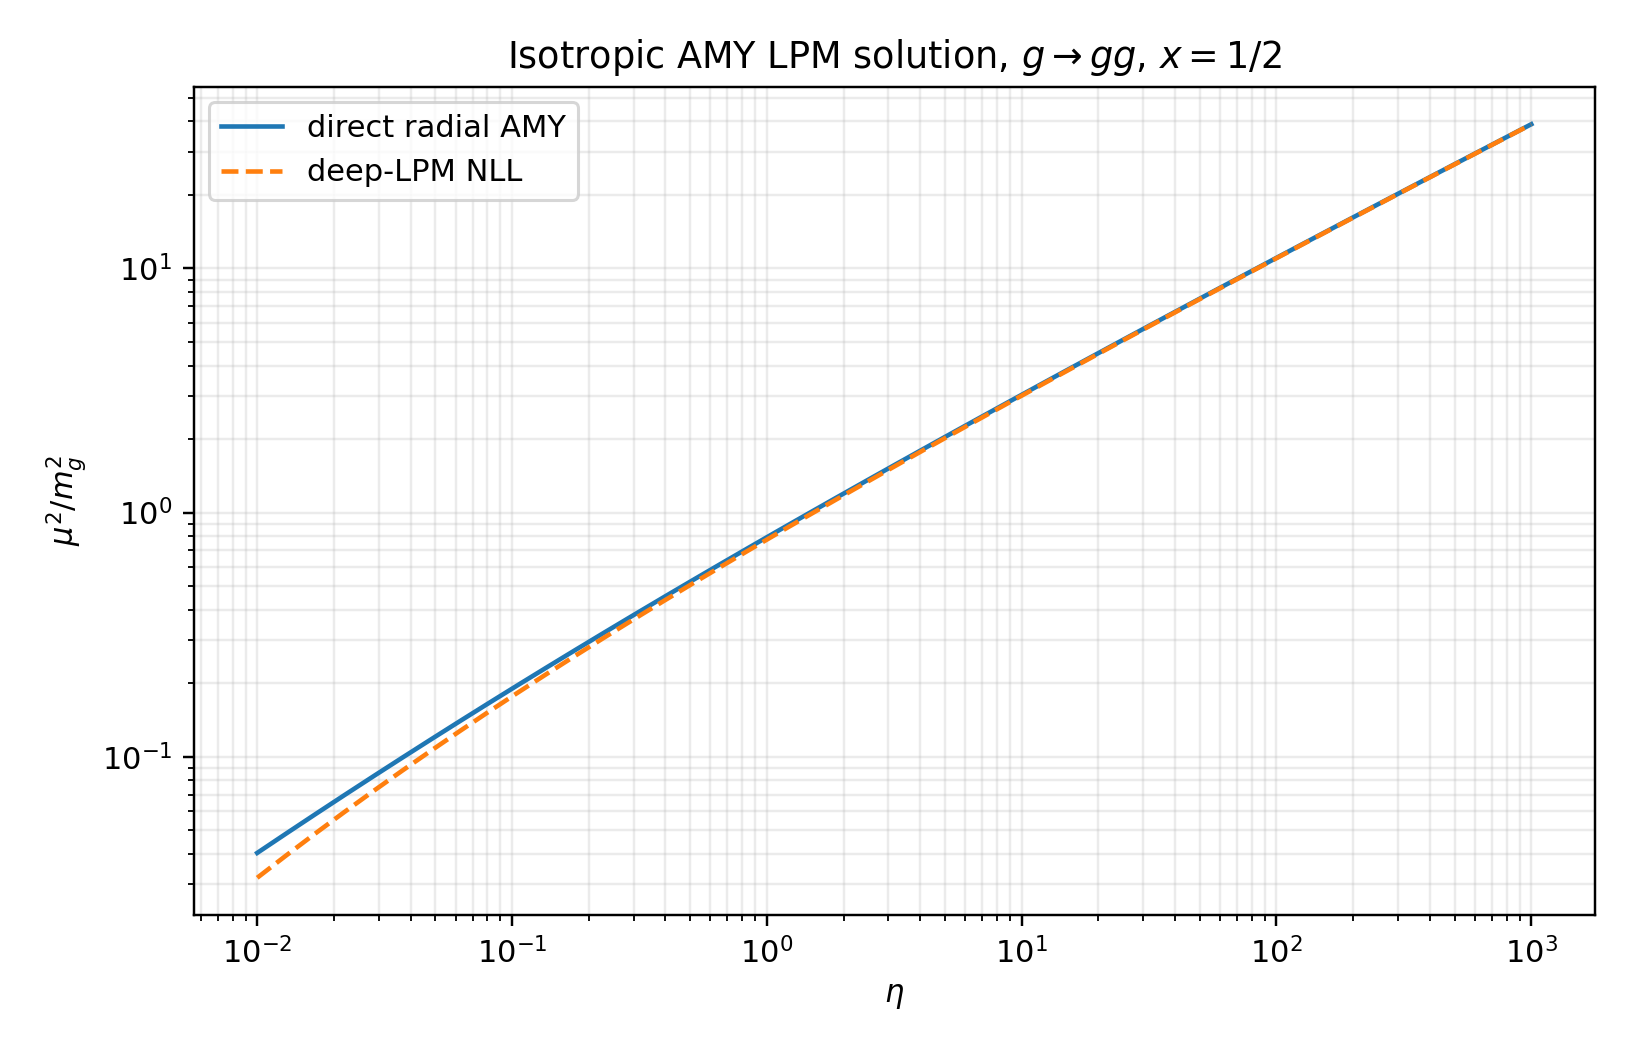
\includegraphics[width=0.88\textwidth,height=\textheight]{amy_lpm_exact_v1_4.png}
\caption{Direct radial AMY solution and deep-LPM comparison.}
\end{figure}

\section{3. Splitting and joining
kernels}\label{splitting-and-joining-kernels}

\subsection{3.1 Gauge splitting rates}\label{gauge-splitting-rates}

The differential rate is reconstructed from the AMY splitting functions.
For example,

\[
\gamma_{gg}^{g}
=
\frac{\sqrt2\,d_A C_A\alpha_s}{(2\pi)^4}
\frac{1+x^4+(1-x)^4}{x^2(1-x)^2}
\mu^2,
\]

and

\[
\frac{d\Gamma_{g\rightarrow gg}}{dx}
=
\frac{(2\pi)^3}{2p\nu_g}
\gamma_{gg}^{g}
[1+f_g(xp)]
[1+f_g((1-x)p)].
\]

For fermion bremsstrahlung,

\[
\gamma_{gq}^{q}
=
\frac{\sqrt2\,d_F C_F\alpha_s}{(2\pi)^4}
\frac{1+(1-x)^2}{x^2(1-x)}
\mu^2.
\]

For pair production,

\[
\gamma_{q\bar q}^{g}
=
\frac{\sqrt2\,d_F C_F\alpha_s}{(2\pi)^4}
\frac{x^2+(1-x)^2}{x(1-x)}
\mu^2.
\]

The numerical table includes

\[
g\leftrightarrow gg,
\qquad
q\leftrightarrow gq,
\qquad
D\leftrightarrow gD,
\]

\[
g\leftrightarrow q\bar q,
\qquad
g\leftrightarrow D\bar D.
\]

\subsection{3.2 Scalar-Yukawa portal
channel}\label{scalar-yukawa-portal-channel}

For

\[
H\leftrightarrow qD,
\]

the parent is colorless and the two daughters are fundamental.
Consequently,

\[
\left(
C_{qD}^{H},
C_{DH}^{q},
C_{Hq}^{D}
\right)
=
\left(
\frac89,0,0
\right).
\]

The direct transverse equation therefore contains one color-dipole
potential. The collinear normalization used in the table is

\[
\frac{d\Gamma_{H\rightarrow qD}}{dx}
=
\frac{N_cy_D^2}{16\pi p}
\mu_{HqD}^2
[1-f_q(xp)]
[1-f_D((1-x)p)].
\]

This channel dominates the slow mode. Because the scalar-Yukawa
prefactor is not one of the original QCD AMY kernels, all cosmological
conclusions are also quoted with the conservative range

\[
\frac12\Gamma_{H\leftrightarrow qD}
<
\Gamma_{H\leftrightarrow qD}^{\rm true}
<
2\Gamma_{H\leftrightarrow qD}.
\]

The hierarchy remains decisive throughout that band.

\section{\texorpdfstring{4. Full-angle screened \(2\leftrightarrow2\)
integral}{4. Full-angle screened 2\textbackslash leftrightarrow2 integral}}\label{full-angle-screened-2leftrightarrow2-integral}

\subsection{4.1 Hard matrix elements}\label{hard-matrix-elements}

The v1.3 angle-averaged leading-log cross section has been replaced by
the screened hard amplitudes used in thermal implementations of AMY
kinetics {[}2{]}. For example,

\[
\frac{|\mathcal M_{gg\rightarrow gg}|^2}{g_s^4}
=
\frac{16d_A C_A^2}{\nu_g^2}
\left[
3
-
\frac{su}{(t-\zeta_gm_g^2)^2}
-
\frac{st}{(u-\zeta_gm_g^2)^2}
-
\frac{tu}{(s+\zeta_gm_g^2)^2}
\right],
\]

with

\[
\zeta_g=\frac{e^{5/3}}{4},
\qquad
\zeta_q=\frac{e^2}{4}.
\]

The calculation includes the full angular dependence of

\[
gg\rightarrow gg,
\qquad
gq\rightarrow gq,
\qquad
qq'\rightarrow qq',
\]

\[
q\bar q\rightarrow gg,
\qquad
gg\rightarrow q\bar q.
\]

\begin{figure}
\centering
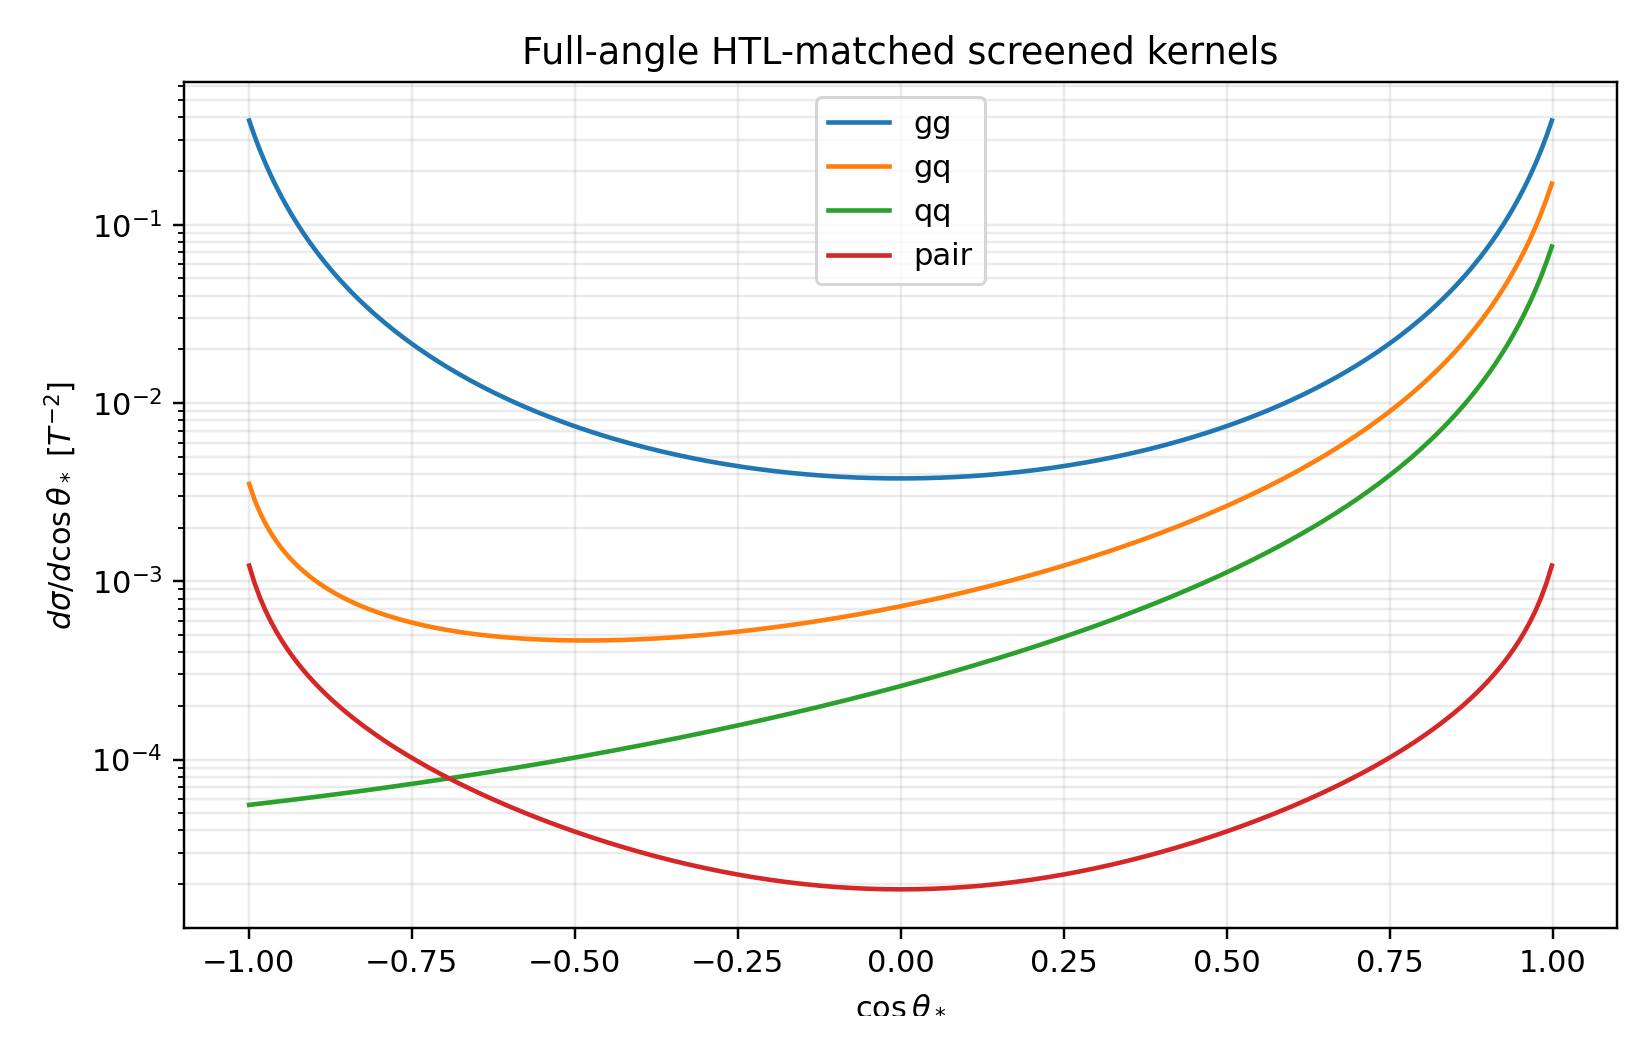
\includegraphics[width=0.88\textwidth,height=\textheight]{amy_full_angle_screened_v1_4.png}
\caption{Representative full-angle screened kernels at \(s/T^2=18\).}
\end{figure}

\subsection{4.2 Thermal transport
moment}\label{thermal-transport-moment}

For a hard test particle of momentum \(p\), the transport moment is
evaluated as

\[
\Gamma_{ab}^{\rm tr}(p)
=
\nu_b
\int
\frac{d^3k}{(2\pi)^3}
 f_b(k)
 v_{\rm rel}
\int d\Omega_*
\frac{d\sigma_{ab}}{d\Omega_*}
(1-\cos\theta_*)
\mathcal Q_{cd},
\]

where

\[
\mathcal Q_{cd}
=
[1\pm f_c(E_c)]
[1\pm f_d(E_d)].
\]

The final energies are calculated by explicitly boosting the outgoing
center-of-momentum four-vectors back into the plasma frame. Thus the
Bose and Pauli factors are angle dependent and are not replaced by a
single fitted number.

At the benchmark,

\[
\frac{\Gamma_{g,\rm elastic}}{T}=0.106177,
\]

and

\[
\frac{\Gamma_{q,\rm elastic}}{T}=0.0119151.
\]

The gluon rate is enhanced by the large gluon channel and by the
multiplicity of quark and antiquark targets.

\section{5. Collision-operator table}\label{collision-operator-table}

\subsection{5.1 Grid}\label{grid}

The integrated table contains 108 rows covering

\[
\alpha_s
\in
\{0.02,0.0393544,0.08\},
\]

\[
\frac{M_D}{T}
\in
\{0,0.01,0.10,0.30\},
\]

\[
y_D
\in
\{0.10,0.30,0.60\},
\]

and

\[
f_a
\in
\{10^9,2.435\times10^{10},10^{12}\}\ \mathrm{GeV}.
\]

The differential NPZ table contains

\[
\frac{p}{T}
\in
\{1.5,3,6,12\},
\]

and

\[
x\in[0.05,0.95]
\]

for all six splitting channels.

\subsection{\texorpdfstring{5.2 Exact \(f_a\)
factorization}{5.2 Exact f\_a factorization}}\label{exact-f_a-factorization}

The local plasma operator depends on dimensionless masses, couplings,
and occupation functions. It contains no independent \(f_a\) argument:

\[
C_{\rm AMY}
=
C_{\rm AMY}
\left[
\frac{M_D}{T},
\alpha_s,
y_D,
f_H,f_D,f_q,f_g
\right].
\]

Therefore,

\[
\boxed{
\left.
\frac{\partial C_{\rm AMY}}
{\partial\ln f_a}
\right|_{M_D/T,\alpha_s,y_D,f_i}
=0.
}
\]

The role of \(f_a\) is upstream:

\[
f_a
\longrightarrow
\text{chronometric-field coupling and source amplitude}
\longrightarrow
\text{initial or external perturbation},
\]

not

\[
f_a
\longrightarrow
\text{QCD thermal transport coefficient}.
\]

This removes one dimension from the intrinsic collision table.

\subsection{5.3 Parameter dependence}\label{parameter-dependence}

The portal rate grows strongly with \(y_D\) and is only mildly modified
by \(M_D/T\) over the relativistic range considered.

\begin{figure}
\centering
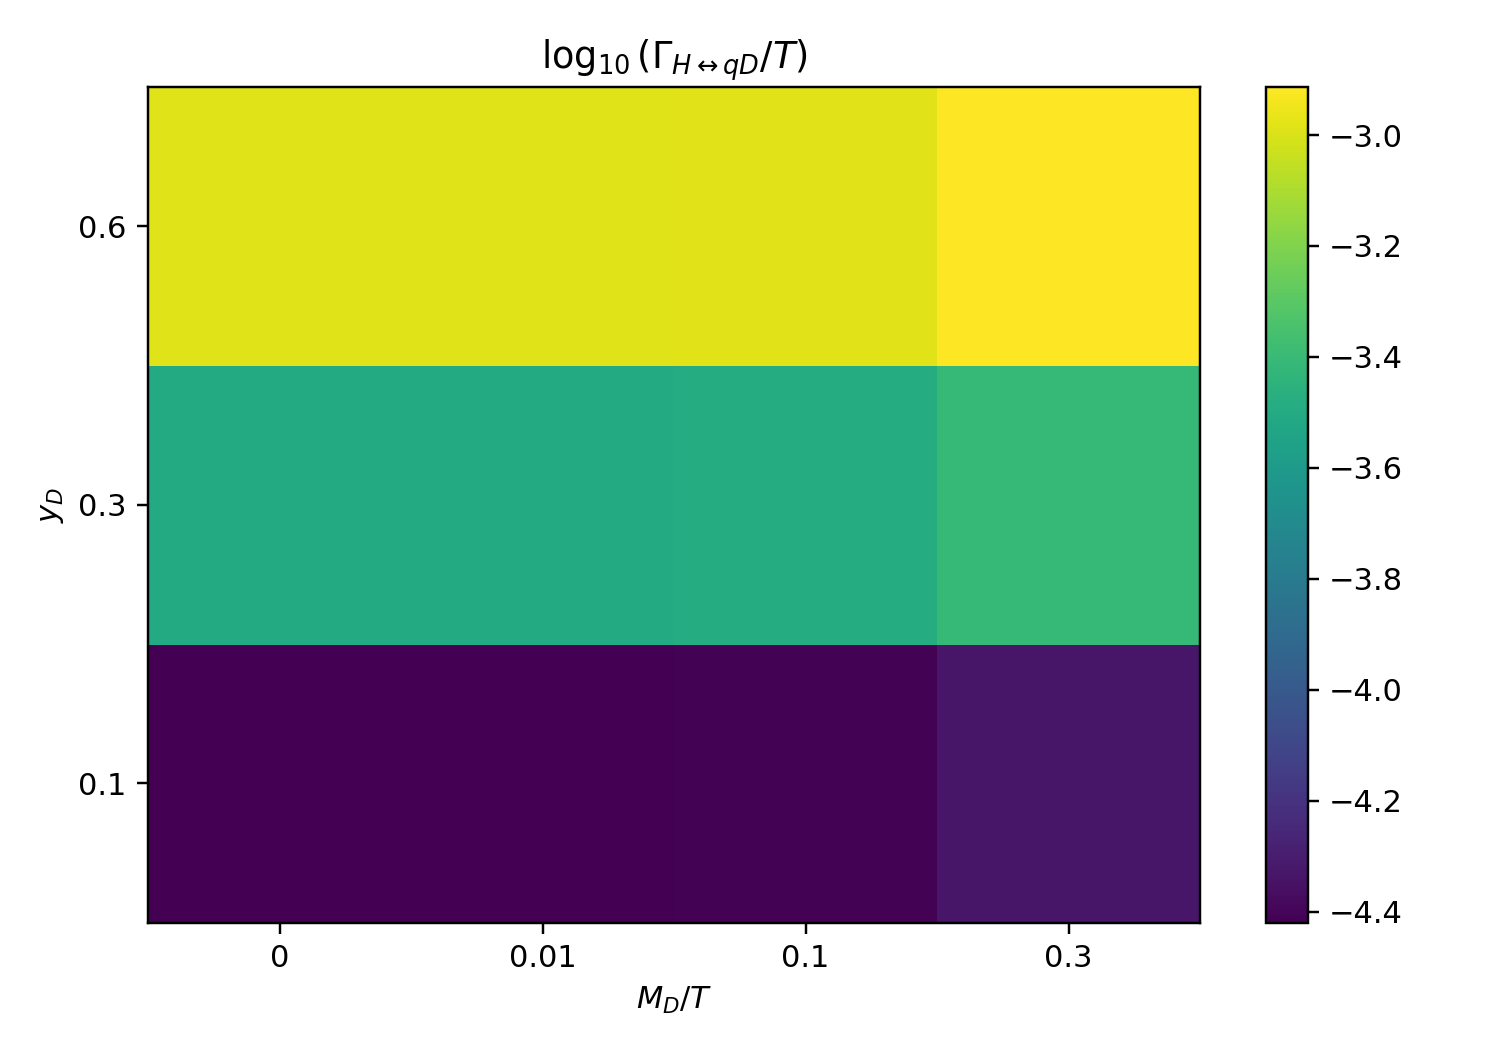
\includegraphics[width=0.76\textwidth,height=\textheight]{amy_parameter_scan_v1_4.png}
\caption{Portal-rate response over \(M_D/T\) and \(y_D\) at the
benchmark strong coupling.}
\end{figure}

Across the scan,

\[
\frac{\Gamma_{H\leftrightarrow qD}}{T}
\in
[1.114\times10^{-5},3.880\times10^{-3}],
\]

and it is the slowest channel in every row.

\section{6. Cosmological cascade
re-run}\label{cosmological-cascade-re-run}

\subsection{6.1 Benchmark hierarchy}\label{benchmark-hierarchy}

The complete benchmark hierarchy is shown below.

\begin{figure}
\centering
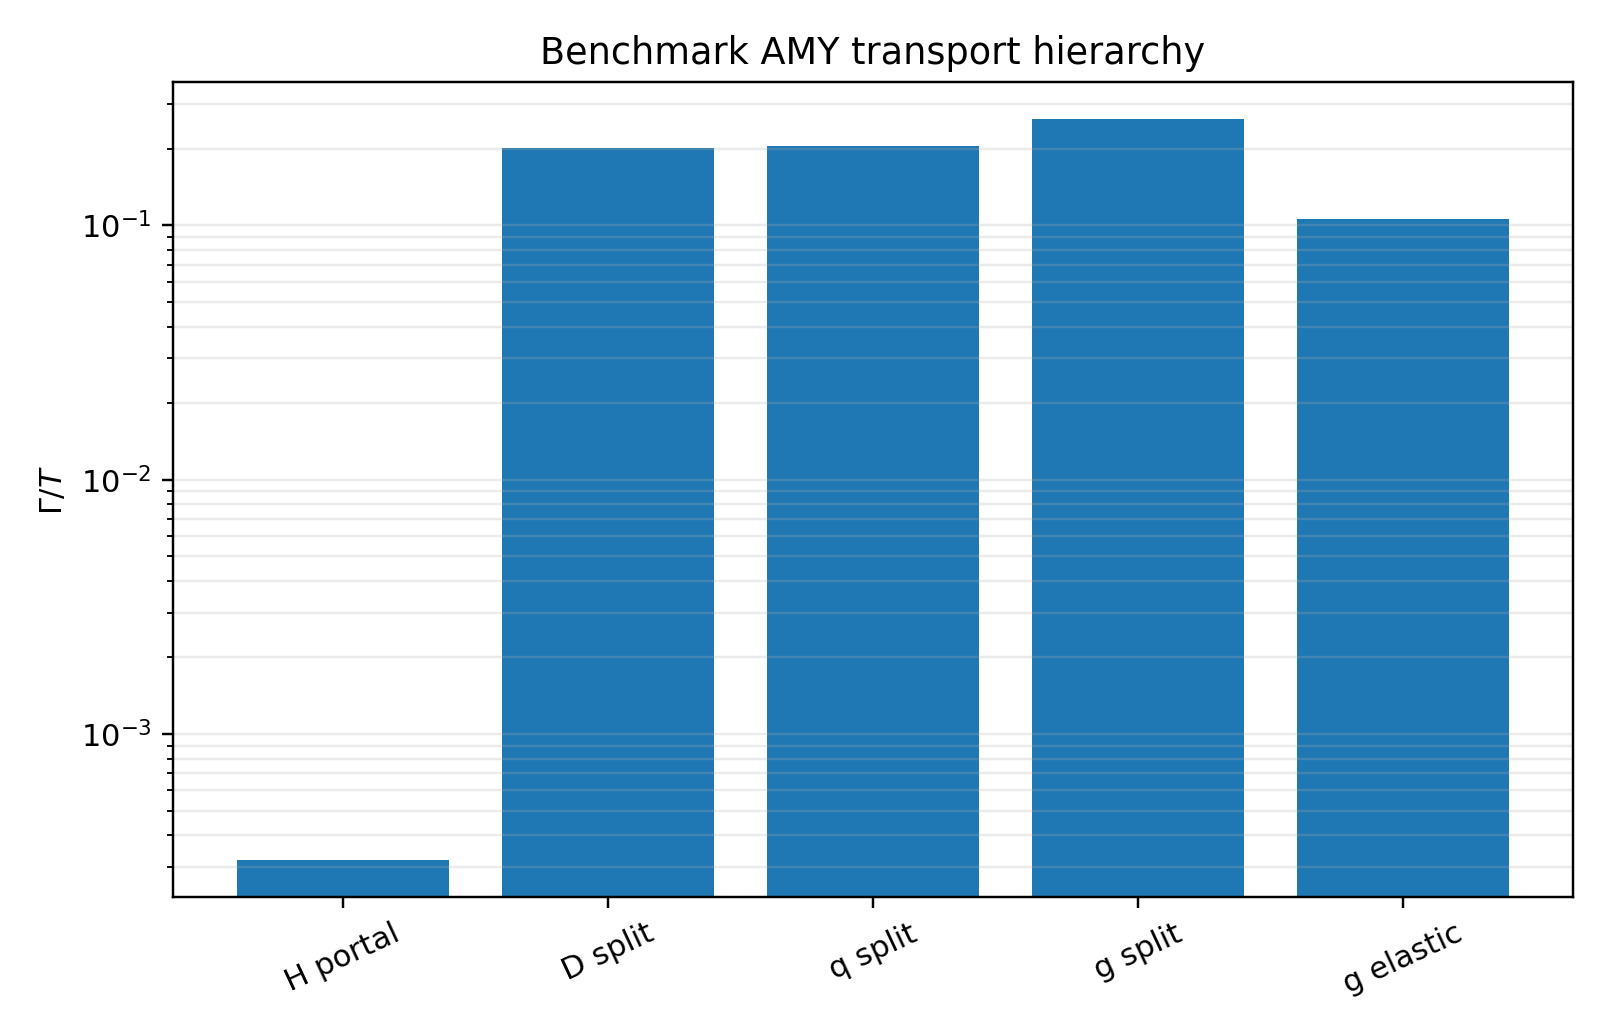
\includegraphics[width=0.78\textwidth,height=\textheight]{amy_rate_hierarchy_v1_4.png}
\caption{Exact-rate hierarchy at \(p/T=3\).}
\end{figure}

The QCD rates are of order

\[
0.1T-0.3T,
\]

while the portal rate is

\[
3.19\times10^{-4}T.
\]

The direct calculation therefore confirms a two-stage cascade:

\[
H
\xrightarrow{\ H\leftrightarrow qD\ }
q,D
\xrightarrow{\rm QCD}
q,D,g\ \mathrm{plasma}.
\]

The first arrow controls the relaxation time. Once energy reaches
colored matter, QCD redistributes it approximately three orders of
magnitude faster.

\subsection{6.2 Why the final temperature ratio does not
move}\label{why-the-final-temperature-ratio-does-not-move}

The collision operator conserves total energy within each replica
sector. Consequently, changing transport coefficients cannot change the
asymptotic sector-energy ratio fixed by reheaton branching, provided all
relevant decay products are relativistic at the epoch of interest.

Finite thermalisation time can affect the result only through the slow
cosmological variation occurring during the lag. The correction scales
as

\[
\delta_{\rm ad}
\sim
\frac{\Gamma_R}{\Gamma_{\rm kin}}.
\]

At the benchmark,

\[
\delta_{\rm ad}=4.63\times10^{-7},
\]

or

\[
\delta_{\rm ad}^{\rm conservative}=9.26\times10^{-7}
\]

using the lower edge of the Yukawa normalization band.

The branching correction is therefore bounded by

\[
|\Delta B_5|
<
B_5\delta_{\rm ad}^{\rm conservative}
=
4.91\times10^{-9}.
\]

Thus the v1.3 values remain

\[
\boxed{
B_5=0.00529888708,
}
\]

and

\[
\boxed{
\frac{T_5}{T_0}=\frac14
}
\]

to the precision relevant for the cosmological analysis.

\subsection{6.3 Robustness over the
scan}\label{robustness-over-the-scan}

At the weakest point in the grid,

\[
\alpha_s=0.02,
\qquad
y_D=0.10,
\qquad
M_D/T=0,
\]

the hierarchy remains

\[
\frac{\Gamma_{\rm kin}}{\Gamma_R}
=7.55\times10^4.
\]

Even after halving the portal rate, the largest possible relative
cascade correction over the table is only

\[
2.65\times10^{-5}.
\]

The conclusion that the plasma thermalizes before the source changes
appreciably is therefore not a peculiarity of one tuned benchmark.

\section{7. AMY-calibrated two-time
benchmark}\label{amy-calibrated-two-time-benchmark}

\subsection{7.1 Reduced memory system}\label{reduced-memory-system}

To prepare a reference for a future non-Abelian 2PI implementation, the
on-shell AMY rate is embedded into a finite-memory system:

\[
\dot n=-2\Gamma y,
\]

\[
\dot y=\Lambda(n-n_{\rm eq})-\Lambda y,
\]

where

\[
\Lambda\sim m_D
\]

sets the environmental memory frequency.

Eliminating \(y\) gives

\[
\ddot n
+
\Lambda\dot n
+
2\Gamma\Lambda(n-n_{\rm eq})
=0.
\]

At the benchmark,

\[
\frac{\Gamma}{\Lambda}
=3.08\times10^{-4}.
\]

The maximum normalized difference between the finite-memory evolution
and its Markov limit is

\[
\boxed{
6.07\times10^{-4}.
}
\]

\begin{figure}
\centering
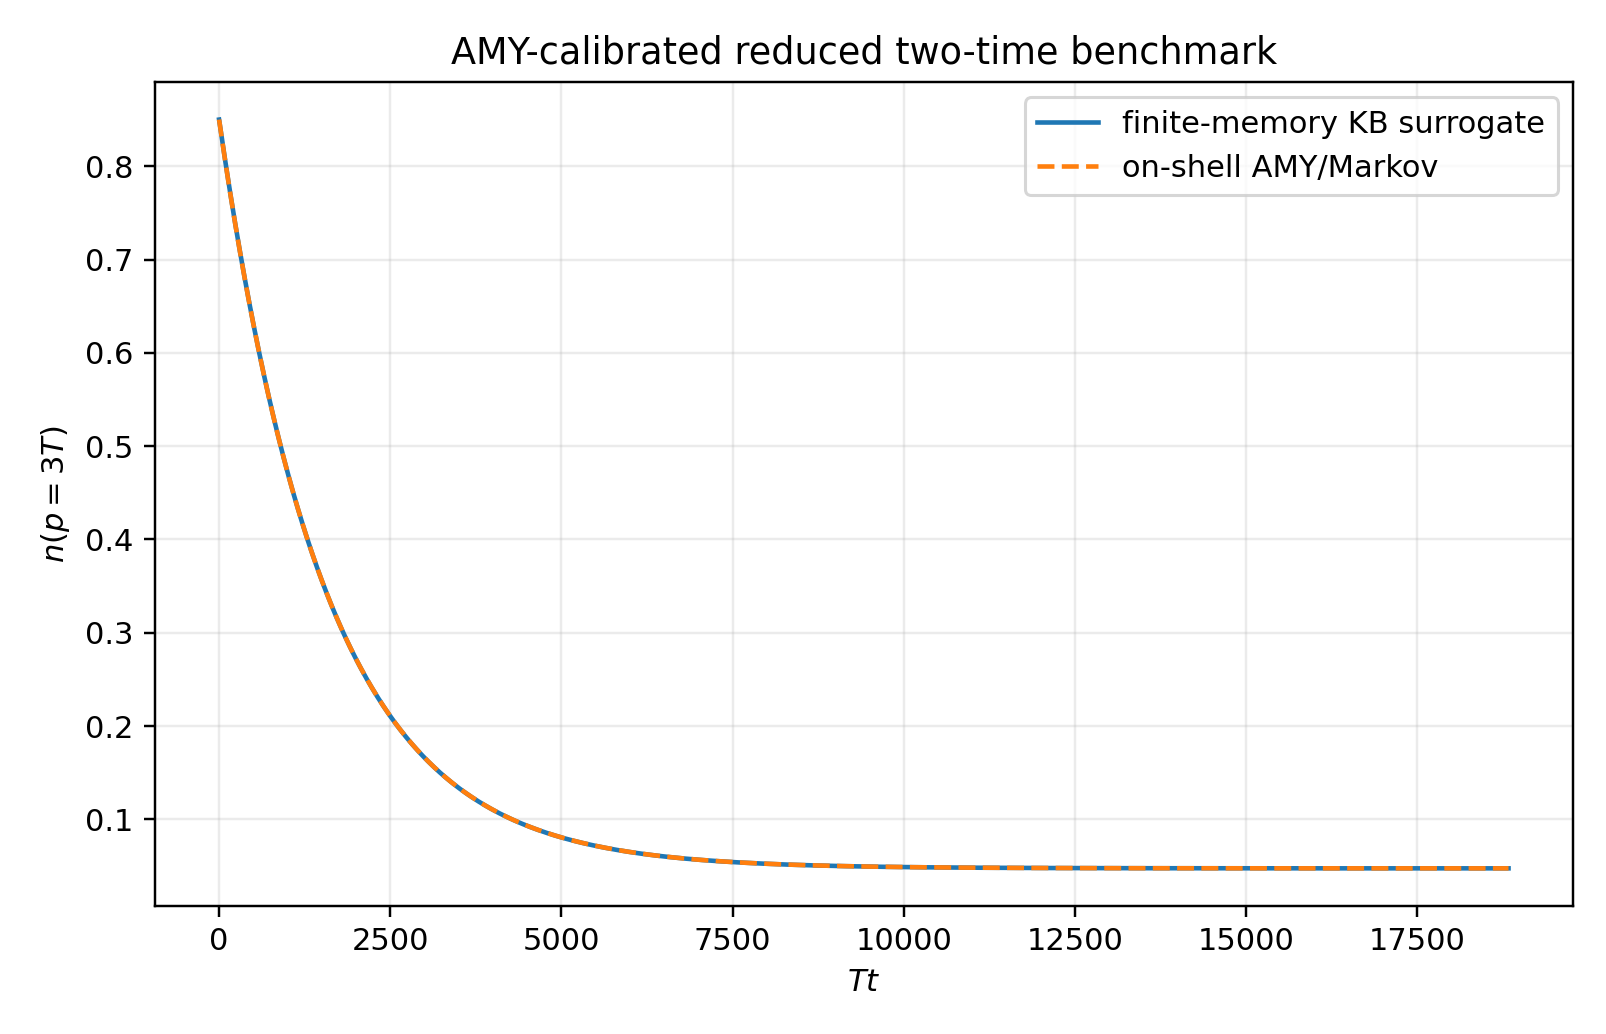
\includegraphics[width=0.84\textwidth,height=\textheight]{amy_reduced_kb_v1_4.png}
\caption{Finite-memory evolution compared with the on-shell AMY limit.}
\end{figure}

\subsection{7.2 Two-time statistical and spectral
functions}\label{two-time-statistical-and-spectral-functions}

The reduced benchmark constructs

\[
\rho(t,t';p)
=
e^{-\Gamma|t-t'|}
\frac{\sin[\omega_p(t-t')]}{\omega_p},
\]

and

\[
F(t,t';p)
=
e^{-\Gamma|t-t'|}
\frac{n((t+t')/2)+1/2}{\omega_p}
\cos[\omega_p(t-t')].
\]

The spectral equal-time normalization gives

\[
\left.
\partial_t\rho(t,t';p)
\right|_{t=t'^+}
=0.999999999895,
\]

consistent with the canonical value 1.

\begin{figure}
\centering
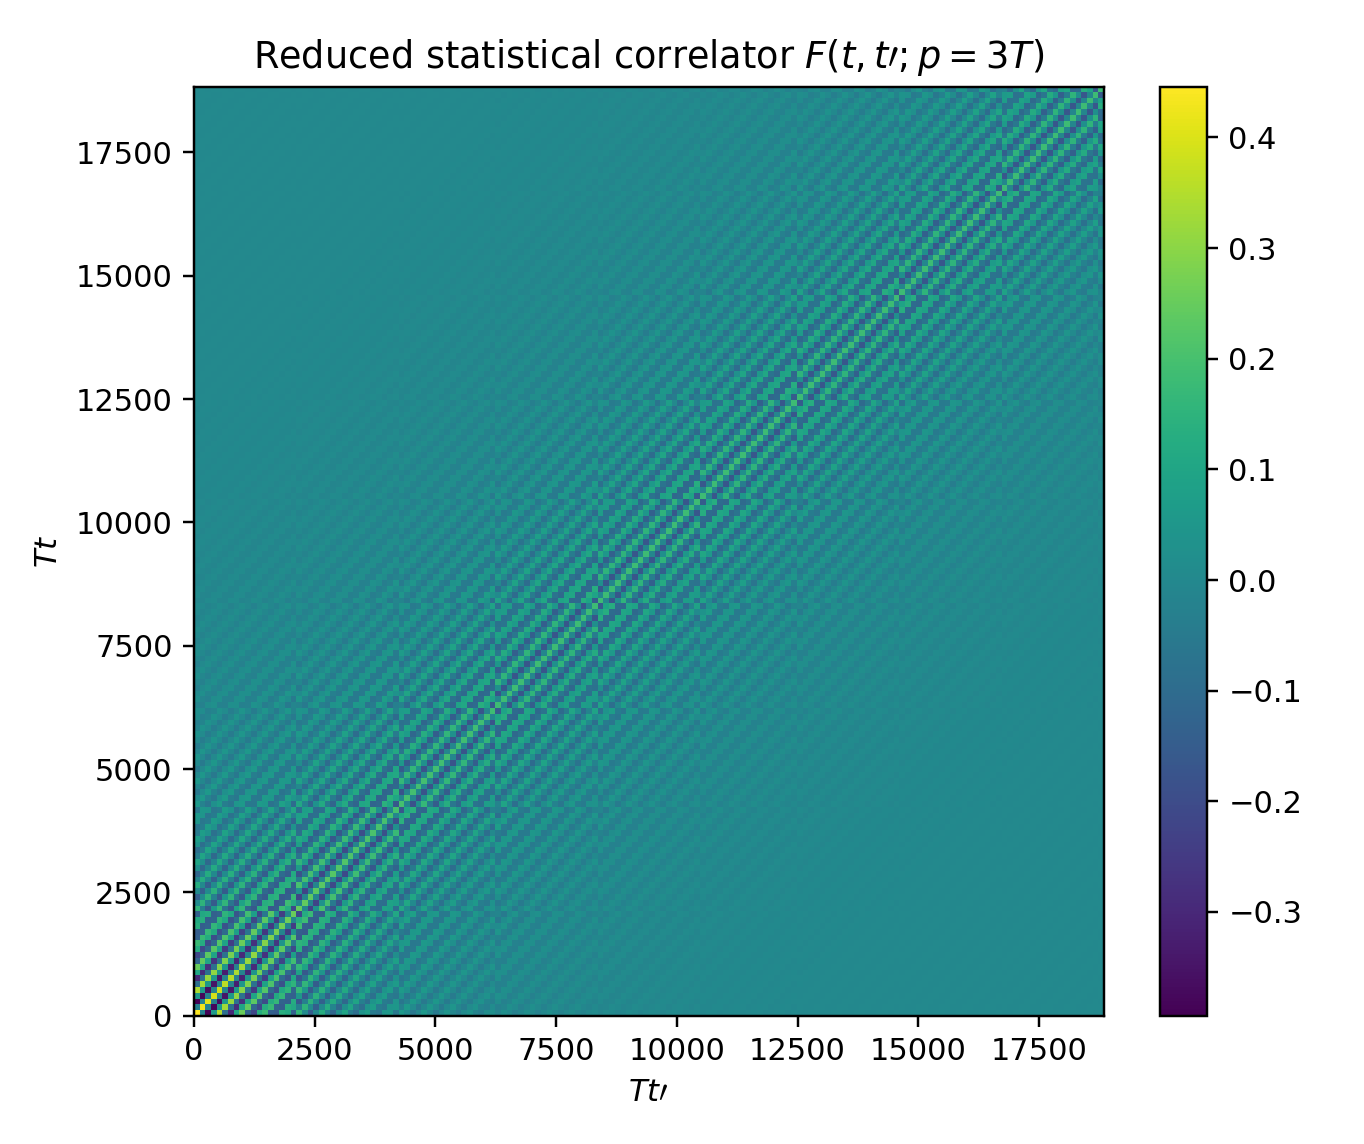
\includegraphics[width=0.78\textwidth,height=\textheight]{amy_two_time_F_v1_4.png}
\caption{Reduced two-time statistical correlator.}
\end{figure}

This construction supplies a concrete numerical target for a future
gauge-theory calculation:

\begin{enumerate}
\def\labelenumi{\arabic{enumi}.}
\tightlist
\item
  the on-shell width must reduce to the AMY rate;
\item
  the spectral equal-time normalization must be preserved;
\item
  the short-memory limit must approach the AMY kinetic trajectory;
\item
  off-shell and memory corrections should be measured relative to the
  \(6\times10^{-4}\) surrogate scale rather than guessed.
\end{enumerate}

\section{8. Interpretation for the chronometric
model}\label{interpretation-for-the-chronometric-model}

The kinetic result cleanly separates three physical layers:

\[
\boxed{
\begin{aligned}
f_a &: \text{sets the chronometric coupling scale},\\
y_D &: \text{controls entry into the colored plasma},\\
\alpha_s &: \text{controls rapid redistribution after entry}.
\end{aligned}
}
\]

The large QCD rates mean that any measurable chronometric shear is not
limited by a failure of the replicated plasma to thermalize. Instead,
the meaningful uncertainties are now:

\begin{itemize}
\tightlist
\item
  the exact scalar-Yukawa LPM normalization;
\item
  the preparation and decay history of the Higgs-like injection channel;
\item
  off-shell corrections in a gauge-covariant two-time theory;
\item
  the mapping from plasma equilibration to late clock and
  equivalence-principle observables.
\end{itemize}

The conceptual risk has therefore moved again:

\[
\boxed{
\text{transport is no longer the fragile part of the construction.}
}
\]

\section{9. Acceptance matrix}\label{acceptance-matrix}

\begin{longtable}[]{@{}
  >{\raggedright\arraybackslash}p{(\columnwidth - 4\tabcolsep) * \real{0.3333}}
  >{\raggedright\arraybackslash}p{(\columnwidth - 4\tabcolsep) * \real{0.3333}}
  >{\raggedright\arraybackslash}p{(\columnwidth - 4\tabcolsep) * \real{0.3333}}@{}}
\toprule\noalign{}
\begin{minipage}[b]{\linewidth}\raggedright
Target
\end{minipage} & \begin{minipage}[b]{\linewidth}\raggedright
Verdict
\end{minipage} & \begin{minipage}[b]{\linewidth}\raggedright
Reason
\end{minipage} \\
\midrule\noalign{}
\endhead
\bottomrule\noalign{}
\endlastfoot
Direct isotropic QCD LPM equation & \textbf{PASS} & Radial
boundary-value solve with asymptotic validation \\
Full-angle screened \(2\leftrightarrow2\) moments & \textbf{PASS} &
Deterministic angular and thermal quadrature \\
Parameter table & \textbf{PASS} & 108 integrated rows and differential
NPZ kernels \\
Intrinsic \(f_a\) dependence & \textbf{FACTORIZES} & No dependence at
fixed dimensionless plasma state \\
\(H\leftrightarrow qD\) normalization & \textbf{PARTIAL} & Direct
transverse solve; scalar prefactor retains factor-two band \\
Cosmological cascade & \textbf{PASS at sector-energy level} & Hierarchy
exceeds \(10^6\) at benchmark \\
Reduced two-time benchmark & \textbf{PASS as surrogate} & AMY-calibrated
memory and two-time functions \\
Full non-Abelian \(3+1\)D 2PI/KB & \textbf{OPEN} & Requires
gauge-covariant HPC evolution \\
\end{longtable}

\section{10. Next decisive calculation}\label{next-decisive-calculation}

The full QCD transport hierarchy is now known well enough that another
brute-force collision refinement has low scientific leverage. The next
decisive target is the portal bottleneck:

\[
\boxed{
\text{full electroweak/Yukawa LPM equation for }H\leftrightarrow qD
}
\]

including:

\begin{enumerate}
\def\labelenumi{\arabic{enumi}.}
\tightlist
\item
  the complete helicity and Higgs-doublet source structure;
\item
  simultaneous \(SU(3)_c\), \(SU(2)_L\), and \(U(1)_Y\) soft collision
  kernels;
\item
  thermal widths and asymptotic masses at the benchmark scale;
\item
  exact matching to the scalar retarded self-energy;
\item
  insertion of that rate into a reduced gauge-covariant
  Schwinger-Keldysh model.
\end{enumerate}

Only after that step is it worth paying the full cost of a non-Abelian
\(3+1\)-dimensional two-time simulation. QCD equilibration is already
approximately three orders of magnitude faster than the portal
bottleneck and more than six orders faster than the cosmological source.

\section{References}\label{references}

\begin{enumerate}
\def\labelenumi{\arabic{enumi}.}
\tightlist
\item
  P. Arnold, G. D. Moore, and L. G. Yaffe, \emph{Effective Kinetic
  Theory for High Temperature Gauge Theories}, arXiv:hep-ph/0209353.
\item
  A. Kurkela, R. Törnkvist, and K. Zapp, \emph{AMY Lorentz Invariant
  Parton Cascade - The Thermal Equilibrium Case}, arXiv:2211.15454.
\item
  P. Arnold, G. D. Moore, and L. G. Yaffe, \emph{Transport Coefficients
  in High Temperature Gauge Theories: (II) Beyond Leading Log},
  arXiv:hep-ph/0302165.
\item
  A. Nishiyama and A. Ohnishi, \emph{Entropy Production in Gluodynamics
  in Temporal Axial Gauge in 2+1 Dimensions}, arXiv:1011.4750.
\item
  Y. Abe and K. Nishii, \emph{Bottom-up Open EFT for Non-Abelian Gauge
  Theory with Dynamical Color Environment}, arXiv:2605.22822.
\end{enumerate}

\end{document}
